\section{Selective Interventions Guided by Representation Changes}
\label{sec:vc-interventions}

Can Adam reach a lower training loss while successive changes in its predictions continue to reverse? Motivated by the large output changes near loss peaks in Fig.~\ref{fig:trace-motion}, we cap the change that Adam's proposed update would produce in each selected unit on fixed reference inputs. Across all three models, this reduced mean training loss even as predictions continued to oscillate.

From Eq.~\eqref{eq:adam-update}, Adam proposes the parameter increment $\Delta\theta_t=-\eta_t d_t$. Let $\Delta\theta_{t,j}^{\ell}$ be the block of this increment for unit $j$ at site $\ell$, including its bias when present. Each row of $H_t^\ell$ contains the inputs to the unit for one reference example or position.\footnote{Each row holds the values under a convolutional filter at one position or, in self-attention, the token representation used to compute its query, key, and value.} We append a column of ones if the unit has a bias. Holding these inputs fixed, the root-mean-square (RMS) change in the unit's response is
\begin{equation}
 s_{t,j}^{\ell}=\frac{\|H_t^\ell\,\Delta\theta_{t,j}^{\ell}\|_2}{\sqrt n}.
 \label{eq:vc-score}
\end{equation}
When this displacement exceeds the site budget $\tau_\ell$, we scale the unit's proposed increment according to
\begin{equation}
 \Delta\theta_{t,j}^{\ell,\mathrm{cap}}
 =\gamma_{t,j}^{\ell}\,\Delta\theta_{t,j}^{\ell},\qquad
 \gamma_{t,j}^{\ell}=\min\!\left(1,\frac{\tau_\ell}{s_{t,j}^{\ell}}\right).
 \label{eq:vc-cap}
\end{equation}
This preserves Adam's proposed direction within each unit. Adam advances its moments before the cap is applied. A zero score or zero calibrated budget gives $\gamma_{t,j}^{\ell}=1$. Updates to earlier layers can also change $H_t^\ell$, so the budget bounds only the unit's direct displacement.

We fix each site's budget at the 25th, 50th, or 75th percentile (q25, q50, or q75) of its unit displacements pooled over the eight Adam updates before treatment. We cap the MLP's two hidden linear maps, all ResNet convolutions, and the Transformer's query, key, value, and feed-forward projections.

\begin{figure*}[!t]
\centering
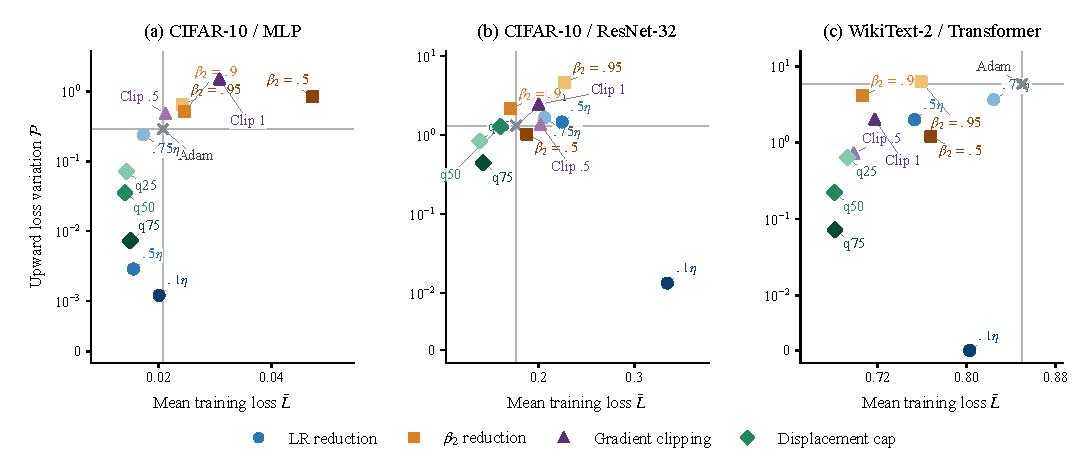
\includegraphics[width=\textwidth]{figures/24-main-intervention-tradeoff.pdf}
\caption{Final training loss and accumulated upward loss variation for unchanged Adam and 11 interventions per model. Points below and to the left of the gray control lines improve both outcomes. The horizontal axis is logarithmic. The vertical axis is linear near zero and logarithmic above $0.001$ for the MLP and $0.01$ for ResNet and the Transformer. Table~\ref{tab:vc-outcomes} gives the settings and absolute outcomes.}
\label{fig:vc-tradeoff}
\end{figure*}

Within each model, every continuation starts from the same parameters, Adam moments, and random state and runs for the same number of full-batch updates (Table~\ref{tab:vc-outcomes}). Alongside unchanged Adam and the three caps, we test learning-rate reductions, reductions in Adam's second-moment coefficient $\beta_2$~\cite{bai2026spikes}, and global gradient clipping~\cite{pascanu2013difficulty}. We report final training loss $L_{t_f}$ and summarize the trajectory from $t_0$ to $t_f$ by its mean loss and accumulated upward loss variation,
\begin{equation}
 \bar L=\frac{1}{t_f-t_0}\sum_{t=t_0+1}^{t_f}L_t,\qquad
 \mathcal P=\sum_{t=t_0+1}^{t_f}\max(L_t-L_{t-1},0).
 \label{eq:vc-outcomes}
\end{equation}

\begin{table*}[!t]
\caption{Absolute matched training outcomes. All numeric outcomes are multiplied by $10^3$; lower is better. Bold marks each column minimum at full precision. Windows are 512--800 (MLP), 256--576 (ResNet), and 544--928 (Transformer), with one initialization per model.}
\label{tab:vc-outcomes}
\centering\fontsize{8.5}{10.5}\selectfont
\setlength{\tabcolsep}{4pt}
\renewcommand{\arraystretch}{1.13}
\begin{tabular}{llrrrrrrrrr}
\toprule
 & & \multicolumn{3}{c}{CIFAR-10 / MLP} & \multicolumn{3}{c}{CIFAR-10 / ResNet-32} & \multicolumn{3}{c}{WikiText-2 / Transformer} \\
\cmidrule(lr){3-5}\cmidrule(lr){6-8}\cmidrule(lr){9-11}
Intervention & Parameter value & $\bar L$ & $\mathcal P$ & $L_{t_f}$ & $\bar L$ & $\mathcal P$ & $L_{t_f}$ & $\bar L$ & $\mathcal P$ & $L_{t_f}$ \\
\midrule
Adam & --- & 20.8 & 288.4 & 30.3 & 176.5 & 1314.9 & 6.7 & 849.6 & 5886.7 & 917.8 \\
\addlinespace[3pt]
\multirow{3}{*}{LR reduction} & $0.75\eta$ & 17.3 & 237.9 & 12.3 & 206.2 & 1662.6 & 21.8 & 824.3 & 3655.5 & 614.0 \\
 & $0.5\eta$ & 15.6 & 2.9 & 10.7 & 224.5 & 1460.9 & 54.5 & 753.1 & 2001.7 & 627.7 \\
 & $0.1\eta$ & 20.1 & \textbf{1.2} & 18.5 & 334.4 & \textbf{13.4} & 244.7 & 802.7 & \textbf{0.0} & 757.2 \\
\addlinespace[3pt]
\multirow{3}{*}{$\beta_2$ reduction} & 0.95 & 24.3 & 648.8 & 19.2 & 226.7 & 4606.1 & 114.2 & 759.0 & 6307.0 & 593.0 \\
 & 0.9 & 24.6 & 513.2 & 15.9 & 170.3 & 2147.5 & 21.4 & 706.5 & 4137.5 & 606.7 \\
 & 0.5 & 47.2 & 829.1 & 34.8 & 187.6 & 1028.9 & 55.1 & 767.8 & 1200.6 & 646.2 \\
\addlinespace[3pt]
\multirow{2}{*}{Gradient clipping} & 0.5 & 21.2 & 476.7 & 16.7 & 202.1 & 1348.5 & 57.8 & 698.5 & 723.3 & 617.0 \\
 & 1 & 30.8 & 1497.6 & 24.4 & 199.9 & 2441.0 & 62.0 & 717.3 & 2027.5 & 620.1 \\
\addlinespace[3pt]
\multirow{3}{*}{Displacement cap} & q25 & 14.4 & 71.2 & 9.7 & \textbf{138.4} & 840.3 & 4.9 & 692.7 & 638.0 & \textbf{550.5} \\
 & q50 & \textbf{14.1} & 35.3 & \textbf{8.7} & 159.9 & 1278.4 & 8.0 & \textbf{681.0} & 221.7 & 703.9 \\
 & q75 & 15.0 & 7.3 & 10.5 & 142.1 & 445.2 & \textbf{4.8} & 681.6 & 72.7 & 583.3 \\
\bottomrule
\end{tabular}
\end{table*}


All three caps lowered mean training loss and accumulated upward variation relative to unchanged Adam in every model (Table~\ref{tab:vc-outcomes}). Among all tested settings, q50 gave the lowest mean loss in the MLP and Transformer, and q25 in ResNet. Smoother trajectories could still end at higher loss (Fig.~\ref{fig:vc-tradeoff}). In ResNet, a tenfold learning-rate reduction cut upward variation by 99\%, yet final loss rose from 0.0067 under unchanged Adam to 0.245. The q25 cap allowed more fluctuation and reached 0.0049. Every tested clipping threshold and $\beta_2$ reduction raised mean loss in the MLP and lowered it in the Transformer.

\begin{figure*}[!tp]
\centering
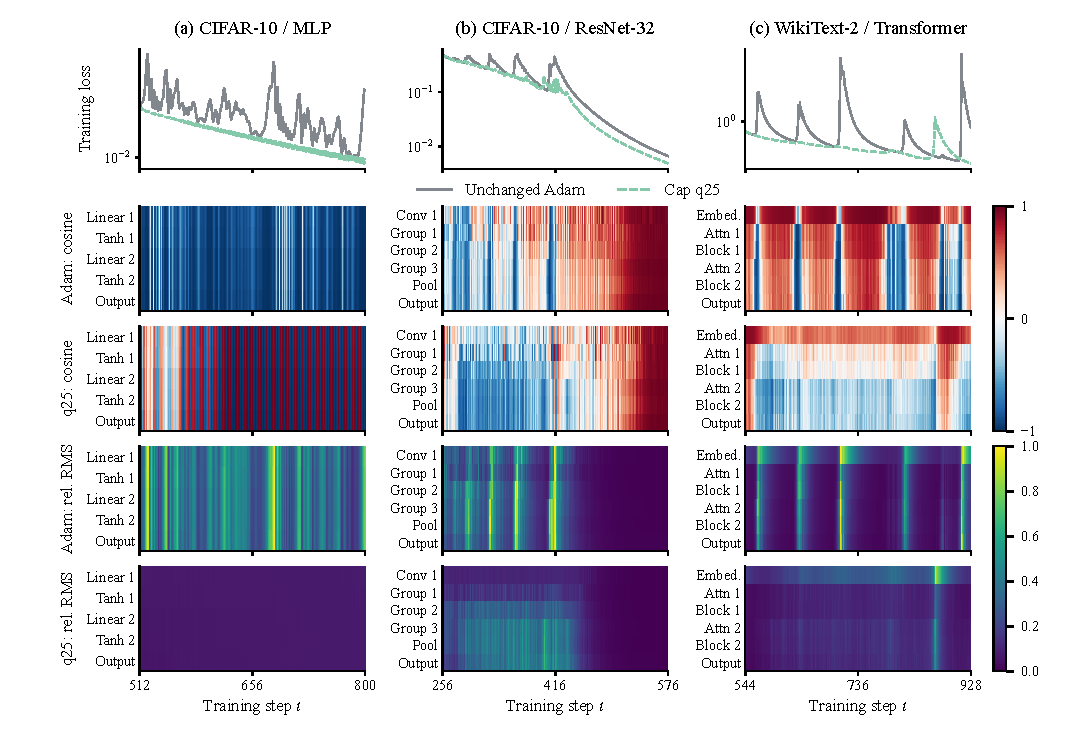
\includegraphics[width=.97\textwidth]{figures/25-main-q25-functional-motion.pdf}
\caption{Unchanged Adam and the q25 displacement cap over the matched continuations. The top row shows full training loss. The paired heatmaps show consecutive-change cosine and RMS displacement on the same reference inputs and at the sites in Fig.~\ref{fig:trace-motion}. Each displacement pair uses the same scale, normalized by the site's maximum under unchanged Adam. Changes are plotted at the completed update.}
\label{fig:vc-motion}
\end{figure*}

Figure~\ref{fig:vc-motion} shows q25 because it lowered all three training metrics in every model. The prespecified q50 setting ended with higher ResNet training loss than unchanged Adam. Under q25, the largest RMS change in predictions fell by 93\% in the MLP, 33\% in ResNet, and 45\% in the Transformer relative to unchanged Adam. Yet consecutive output changes still reversed on 50\%, 60\%, and 89\% of updates, respectively.

The MLP's squared-error loss explains how an output change can point toward the targets and still increase loss. Let $\widehat Y_t$ and $Y$ be the prediction and target matrices on all $N=5000$ training examples, and let $\Delta\widehat Y_t=\widehat Y_{t+1}-\widehat Y_t$. The loss change is exactly
\begin{equation}
 L_{t+1}-L_t=\frac{\langle\widehat Y_t-Y,\Delta\widehat Y_t\rangle_{\mathrm{F}}}{N}
              +\frac{\|\Delta\widehat Y_t\|_{\mathrm{F}}^2}{2N}.
 \label{eq:vc-output-loss}
\end{equation}
Here $\langle A,B\rangle_{\mathrm{F}}=\sum_{i,j}A_{ij}B_{ij}$ is the Frobenius inner product.
Among loss increases exceeding $10^{-8}$, the first term was negative in all 161 cases under unchanged Adam and in 139 of 140 under q25. In each of these cases the output moved toward correcting the current error, but the positive squared-displacement term outweighed that gain. The inner product here measures alignment with the current error, whereas the cosine in Fig.~\ref{fig:vc-motion} measures alignment with the preceding output change.

In these matched runs, limiting large local changes made functional reversal less disruptive to training. The comparison covers one initialization per model at a fixed update budget. The lower loss at that budget came with additional computational cost. In the MLP, computing the q50 cap took 41.8~ms per update, compared with 4.4~ms for the full gradient.
